\section{基準となるロボットの解析}\label{ux57faux6e96ux3068ux306aux308bux30edux30dcux30c3ux30c8ux306eux89e3ux6790}

ここでは,基準となるロボットアームの解析を行う.

解析手順としては以下の手順で行った.

\begin{enumerate}
\def\labelenumi{\arabic{enumi}.}
\item
  Soild
  Edgeを使って,質量や慣性モーメントを求め,解析的に求めた値を比較する
\item
  Solid Edgeを使って,応力をかけた状況をシミュレーションする.
\item
  解析に必要な座標系を定義し,DH記法を用いてリンクパラメータを整理する
\item
  SimXpertを使用して関節加速度及び手先角速度を調べ,解析的に求めた値と比較する
\end{enumerate}

\subsection{基準ロボットの構造解析}\label{ux57faux6e96ux30edux30dcux30c3ux30c8ux306eux69cbux9020ux89e3ux6790}

ここでは,基準となるロボットアームの構造解析を行う.慣性モーメント,応力,変位に関してそれぞれシミュレーションを行い,理論解との照らし合わせてシミュレーション結果の妥当性を考える.

\subsubsection{慣性モーメントの解析}\label{ux6163ux6027ux30e2ux30fcux30e1ux30f3ux30c8ux306eux89e3ux6790}

SolidEdgeを使って求めたリンクアームの体積,質量,慣性モーメントに加え,材質と密度をまとめて記載したものが表\ref{basis-robot-data}である.有効数字は4桁とした.

\begin{table}[htb]
\caption[]{リンクアームの各値}
  \begin{center}
    \begin{tabular}{|c|c|} \hline
      材質 & アルミニウム1060 \\ \hline
      密度 [$\rm kg/m^3$]& 2712 \\ \hline
      体積[$\rm m^3$] & 0.1792 \\ \hline
      質量[kg] & 485.8 \\ \hline
      慣性モーメント[$\rm kg m^2$] & 751.9  \\ \hline
    \end{tabular}
    \label{basis-robot-data}
  \end{center}
\end{table}

ここで,Solid
Edgeによって得た慣性モーメントの値を,解析的に計算した慣性モーメントの値と比較する.

任意の軸回りの慣性モーメント\(I\)は,重心を通る回転軸周りの慣性モーメント\(I_G\)と,2つの軸間距離\(d\),そして質量Mを使うと,平行軸の定理より式\ref{heiko}が成り立つ.

\begin{eqnarray}
  I &=& I_G+d^2M
  \label{heiko}
\end{eqnarray}

また,重心を通る\(Z\)軸周りの直方体の慣性モーメント\(I_G\)は,\(X\)方向の直方体の長さを\(2a\),\(Y\)方向の直方体の長さを\(2b\)とした時に,式\ref{kansei}が成り立つ

\begin{eqnarray}
  I_G &=& \frac{1}{3}M(a^2+b^2)
  \label{kansei}
\end{eqnarray}

図\ref{default-robot-arm}で示した,基準アームを直方体として考えると,\(X\)方向の直方体の長さ\(2a\)は\(0.2\){[}m{]},\(Y\)方向の直方体の長さ\(2b\)は\(2.4\){[}m{]}となる.

よって,\(a=0.1\),\(b=1.2\)となり,質量M=485.832であるので,これらを式\ref{kansei}に代入すると,式\ref{solveBasisKanseiG}のようになる.

\begin{eqnarray}
  I_G &=& \frac{1}{3}M(a^2+b^2) \nonumber \\
&=& \frac{1}{3} 485.8(0.1^{2}+1.2^{2}) \nonumber \\
      &=& 234.8
  \label{solveBasisKanseiG}
\end{eqnarray}

質量中心周りに座標系を定義し,その座標軸周りの慣性モーメント\(I_G\)をSolidEdgeを使用して測った所,225.9{[}\(\rm kg m^2\){]}となっており,解析的に求めた重心周りの慣性モーメント\(I_G\)と数値的に求めた重心周りの慣性モーメント\(I_G\)がほぼ一致している.

慣性モーメントの理論値を求める際は,単純化のために直方体として扱かったため,ブレードを取り付けるために開けた穴及びフィレットを考慮していない.結果的に,理論値がSolidEdgeを使って求めた慣性モーメントと比較して大きく出たと考えられる.

また,回転中心の軸とアームの重心の軸はSolid
Edgeを使用して計測した結果,1.036{[}m{]}の距離があることがわかった.そこで,軸間距離\(d=1.036[\rm m]\),先ほど数値的に計算した重心周りの慣性モーメント\(I_G=234.8[\rm kgm^2]\)及び質量\(M=485.8[\rm kg]\)を式\ref{kansei}に代入すると,式\ref{solveBasisKansei}となる.

\begin{eqnarray}
  I &=& I_G+d^2M \nonumber \\
    &=& 234.8 + 1.036^{2} 485.8 \nonumber \\
    &=& 756.0 
  \label{solveBasisKansei}
\end{eqnarray}

となり,Solid
Edgeを使って解析的に求めた慣性モーメントの値751.9{[}\(\rm kg m^2\){]}とほぼ一致する事がわかる.
ここで発生した誤差も,先ほどの重軸回りの慣性モーメントを求めたときと同様に同様にアームを直方体として直方体として扱ったために生じたものだと考えられる.

次に,リンクアームの先端部分及び中心部分のブレッドを取り付ける部分に117.72{[}N{]}の荷重,及びリンクアームの自重をかけて構造解析を行った.

\subsubsection{応力の解析}\label{ux5fdcux529bux306eux89e3ux6790}

基準となるリンクアームの応力図を図\ref{basis-ouryoku}に示す.

\begin{figure}[htbp]
  \begin{center}
    \begin{tabular}{c}
      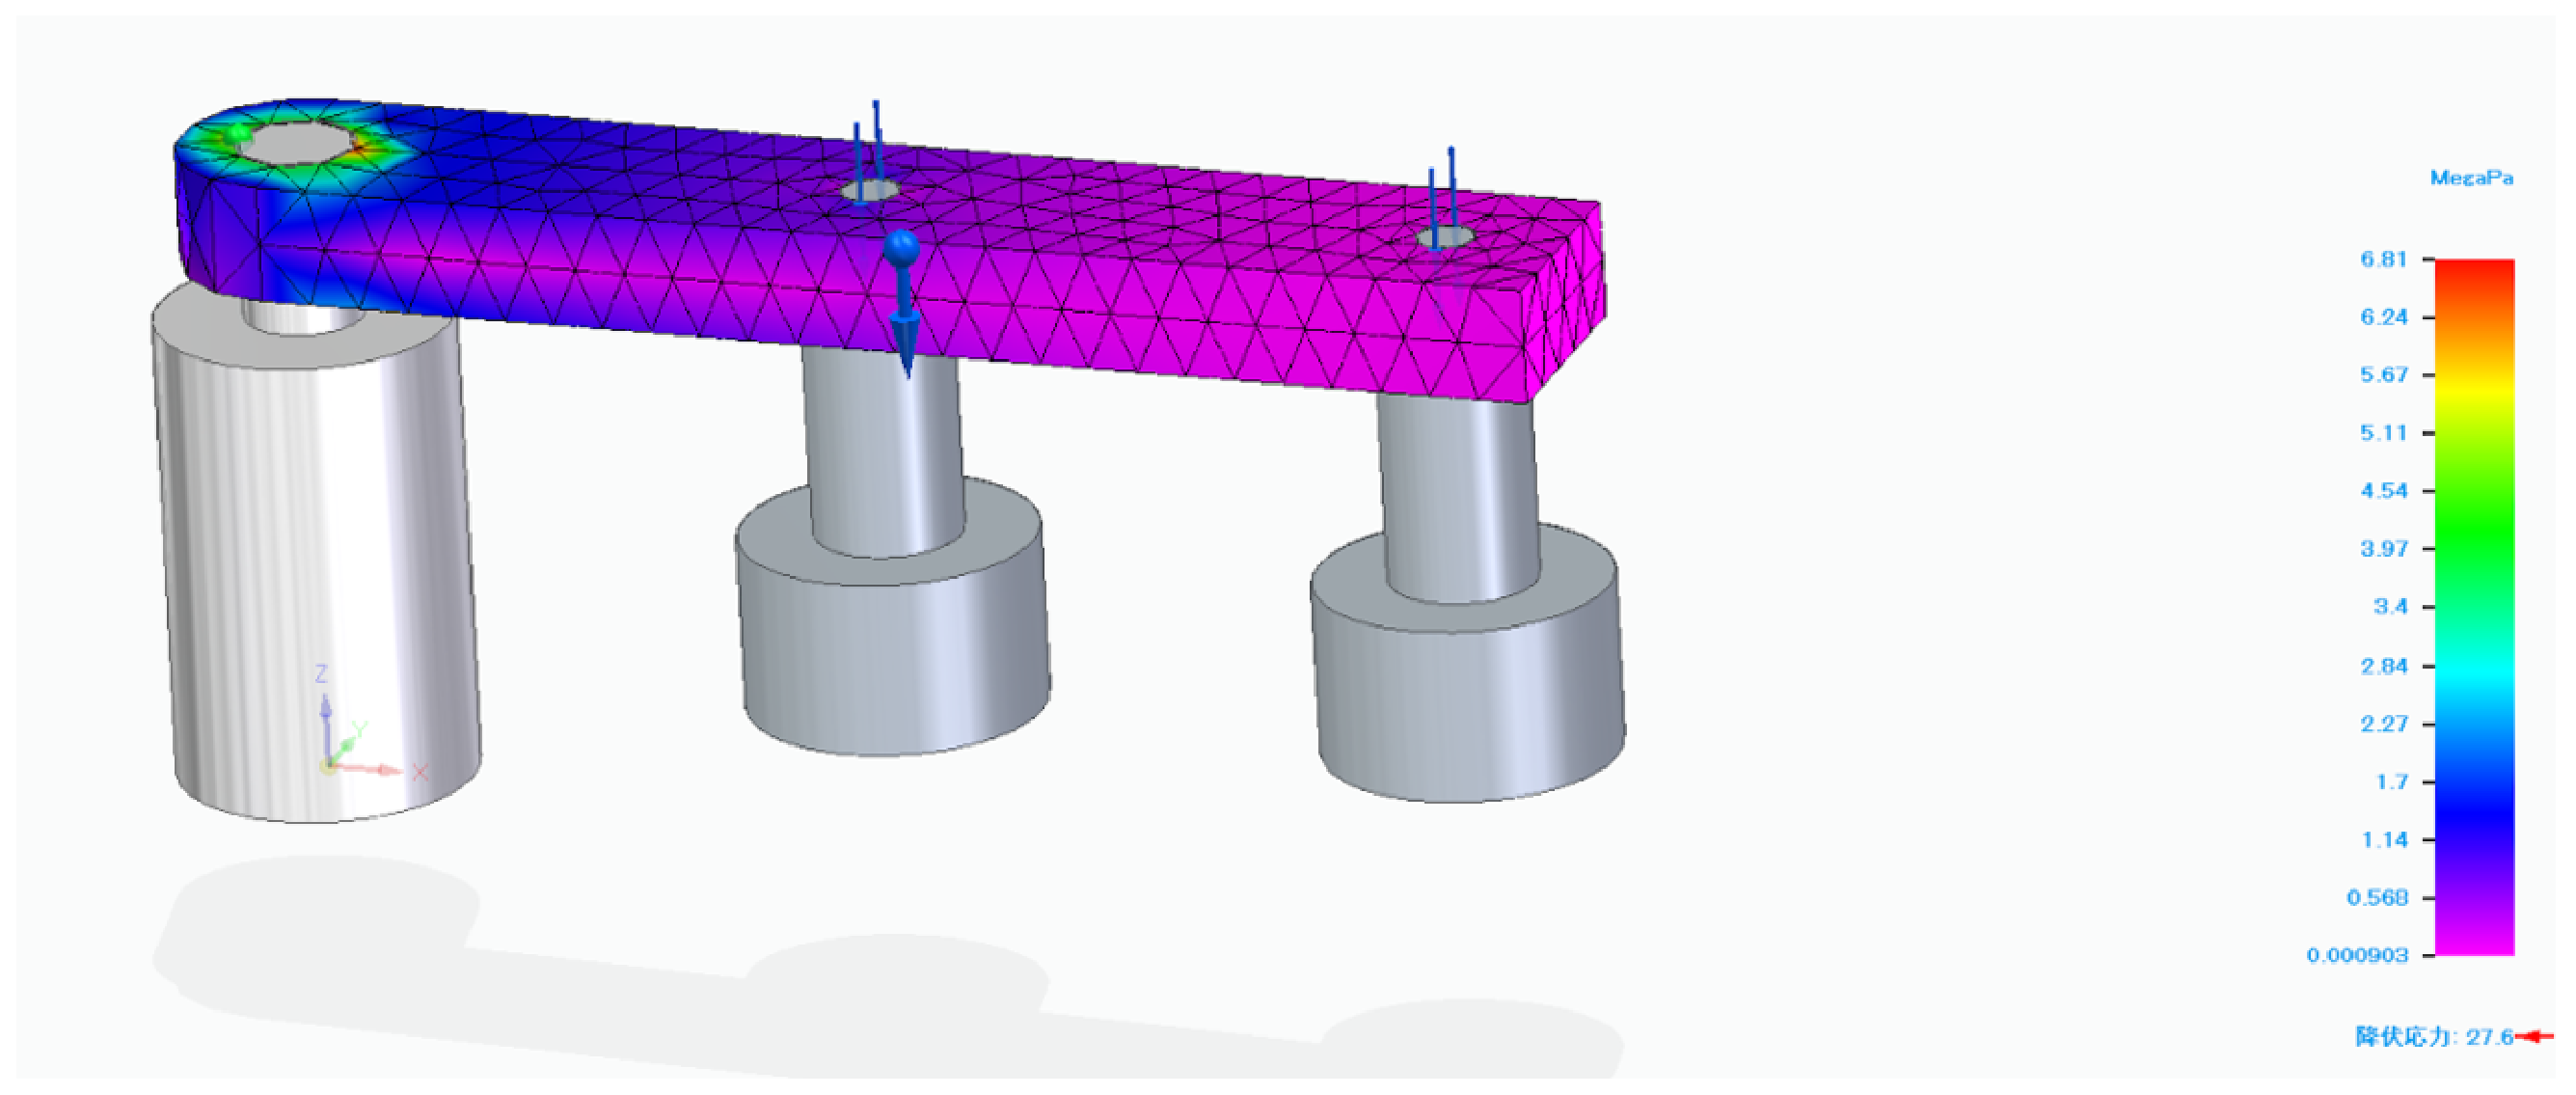
\includegraphics[height=5.5cm]{img/eps/basis-ouryoku.eps}
    \end{tabular}
    \caption{基準ロボットの応力図}
    \label{basis-ouryoku}
  \end{center}
\end{figure}

この応力図の結果より,アームの根元部分に大きな応力がかかっているということがわかった.
この時,図\ref{default-ouryoku-result}に示す結果がSolid
Edgeより出力された.

\begin{figure}[htbp]
  \begin{center}
    \begin{tabular}{c}
      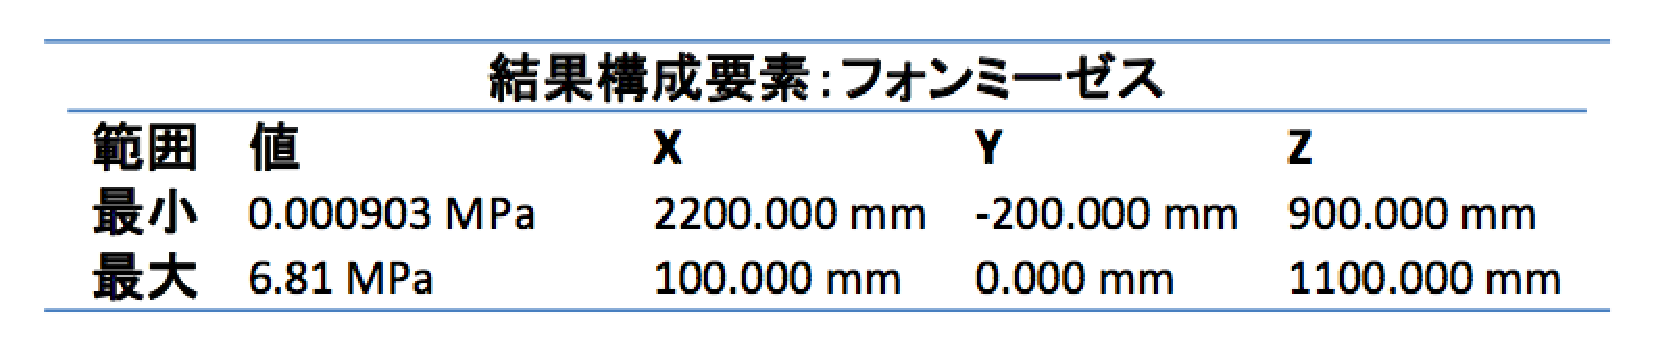
\includegraphics[height=2.5cm]{img/eps/default-ouryoku-result.eps}
    \end{tabular}
    \caption{基準ロボットの応力解析結果}
    \label{default-ouryoku-result}
  \end{center}
\end{figure}

Solid Edgeによって得た応力の結果と,応力の理論値を比較する.

アームの自重を\(M_{arm}\),回転軸とアームの重心点の距離を\(R_a\),アーム中心部に設置されたブレードの荷重による力を\(F_1\),回転軸とアームの中心部の距離を\(R_{b1}\),アーム先端に設置されたブレードの荷重による力を\(F_2\),回転軸とアーム先端部の距離を\(R_{b2}\)とすると,アームの部分にかかる曲げモーメント\(M\)は式\ref{default-magemoment}で表される.
ただし,重力加速度は\(g\)と置いた.

\begin{eqnarray}
  M &=& M_{arm}g R_a + F_1 R_{b1} + F_2 R_{b2} 
  \label{default-magemoment}
\end{eqnarray}

今回,アームの重さが485.832{[}kg{]}であるので,\(M_{arm}=485.8\),\(g=9.81\),\(R_a=1.036\),\(F_1=F_2=117.7\),\(R_{b1}=1\),\(R_{b2}=2\)を代入すると,式\ref{default-magemoment-calc}となる.このとき,\(R_a\)は先ほど求めた回転軸と重心の軸間距離を使用した.

\begin{eqnarray}
  M &=& M_{arm}g R_a + F_1 R_{b1} + F_2 R_{b2}  \nonumber \\
    &=& 485.8*9.81*1.036 + 1*117.7+2*117.7 \nonumber \\
    &=& 5114
  \label{default-magemoment-calc}
\end{eqnarray}

となるので,曲げモーメントMは5114{[}\(\rm kg m^2\){]}となる.

ここで,応力\(\sigma\)は,断面係数\(Z\)を用いて,式\ref{default-ouryoku}と書ける.

\begin{eqnarray}
  \sigma &=& \frac{M}{Z}
  \label{default-ouryoku}
\end{eqnarray}

また,断面係数Zは,直方体のY方向長さ\(b\)と,直方体のZ方向長さ\(h\)を使って,式\ref{default-danmen}と書ける.

\begin{eqnarray}
  Z &=& \frac{bh^2}{6}
  \label{default-danmen}
\end{eqnarray}

今回,\(b=0.4[\rm m]\),\(h=0.2[\rm m]\)であるので,式\ref{default-danmen}より,式\ref{default-danmen-calc}と計算できる.

\begin{eqnarray}
  Z &=& \frac{bh^2}{6} \nonumber \\
    &=& \frac{0.4*0.2^2}{6} \nonumber \\
    &=& 0.002667
  \label{default-danmen-calc}
\end{eqnarray}

求めた曲げモーメント\(M\)及び断面係数\(Z\)を式\ref{default-ouryoku}に代入し,応力を求めると式\ref{default-ouryoku-calc}となる.

\begin{eqnarray}
  \sigma &=& \frac{M}{Z} \nonumber \\
         &=& \frac{5114.3}{0.002667} \nonumber \\
         &=& 1917528 [\rm Pa]\nonumber \\
         &=& 1.92 [\rm MPa]
  \label{default-ouryoku-calc}
\end{eqnarray}

となる.ただしこれは,穴が空いていない場合の応力の値である.

中心部における穴の空いていない部分は,図\ref{basis-ouryoku}の応力分布をみると青く表示されており,約1.9{[}MPa{]}の応力がかかっていることが分かる.ゆえに,この解析結果は正しいと分かる.

穴が開いている部分に関しては,応力集中が起こるため,先ほど計算した穴が空いていない場合にかかる応力よりも大きくなる.穴の周辺で応力が大きくなっていることが図\ref{basis-ouryoku}から読み取れる.

さらに,穴の周辺での最大応力は,穴が空いていない部分応力の約3〜4倍になることが知られており,Solid
Edgeによって得られた最大応力6.81{[}MPa{]}という値も正しいということが分かる.

今回した素材である,アルミニウム1060の降伏応力は27.6{[}MPa{]}であるので,安全率は3を満たすためには,式\ref{basic-anzen}より,許容応力が9.2{[}Mpa{]}であることが分かる.

\begin{eqnarray}
  許容応力 &=& \frac{降伏応力}{安全率} = 9.2[\rm MPa]
  \label{basic-anzen}
\end{eqnarray}

今回,最大応力は6.81{[}MPa{]}であり,許容応力以下であるため安全率3の基準を満たしているといえる.

\subsubsection{変位の解析}\label{ux5909ux4f4dux306eux89e3ux6790}

次に,重力及び荷重によってかかる変位について解析する.

Solid
Edgeのシミュレーション機能を用いて変位を解析した所,変位分布は図\ref{basis-heni}となった.

\begin{figure}[htbp]
  \begin{center}
    \begin{tabular}{c}
      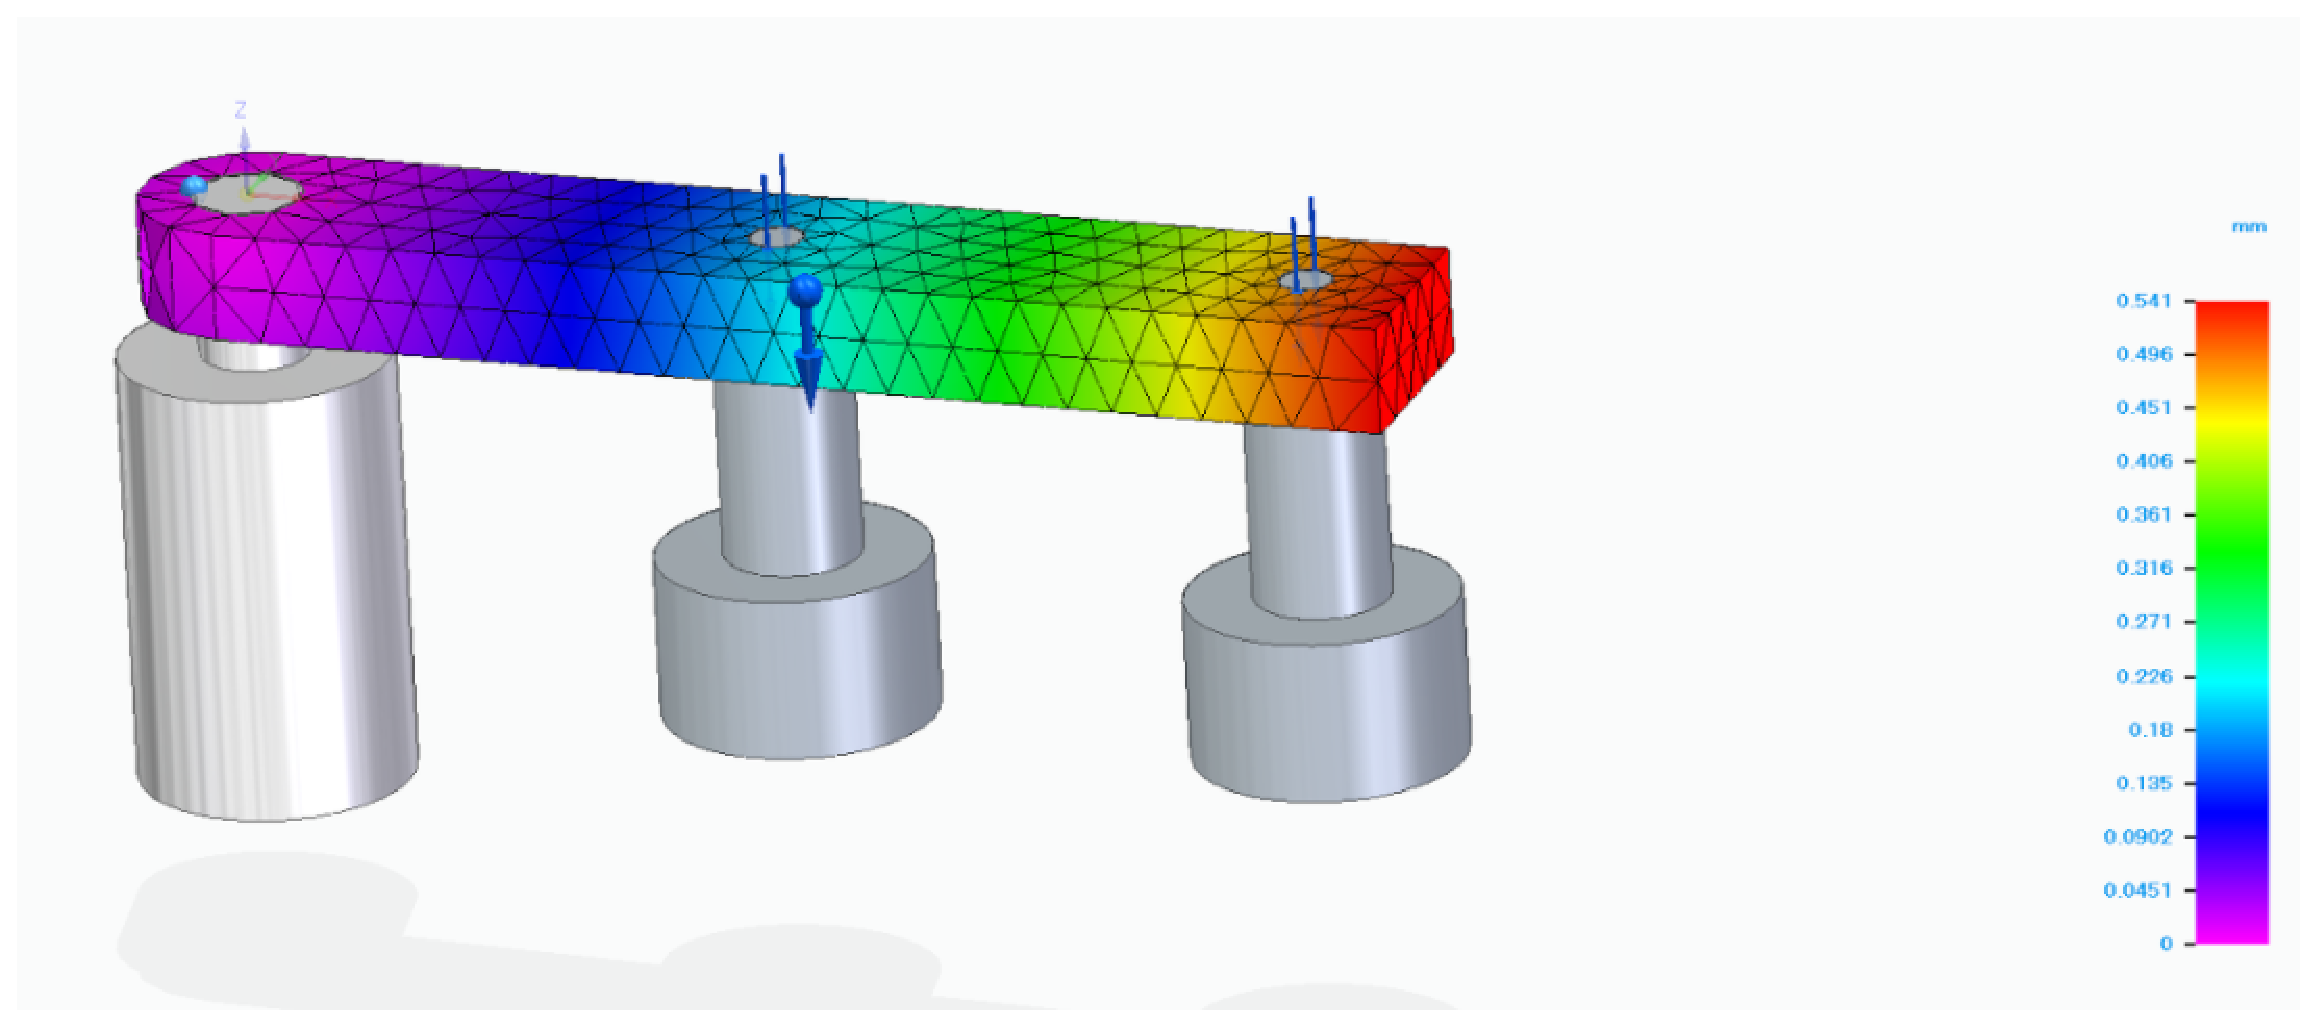
\includegraphics[height=5.7cm]{img/eps/default-heni.eps}
    \end{tabular}
    \caption{基準ロボットの変位分布}
    \label{basis-heni}
  \end{center}
\end{figure}

この応力図の結果より,アームの先端部分に大きな変位が生じることがわかった.

この時,図\ref{default-heni-result}に示す変位結果がSolid
Edgeより出力された.

\begin{figure}[htbp]
  \begin{center}
    \begin{tabular}{c}
      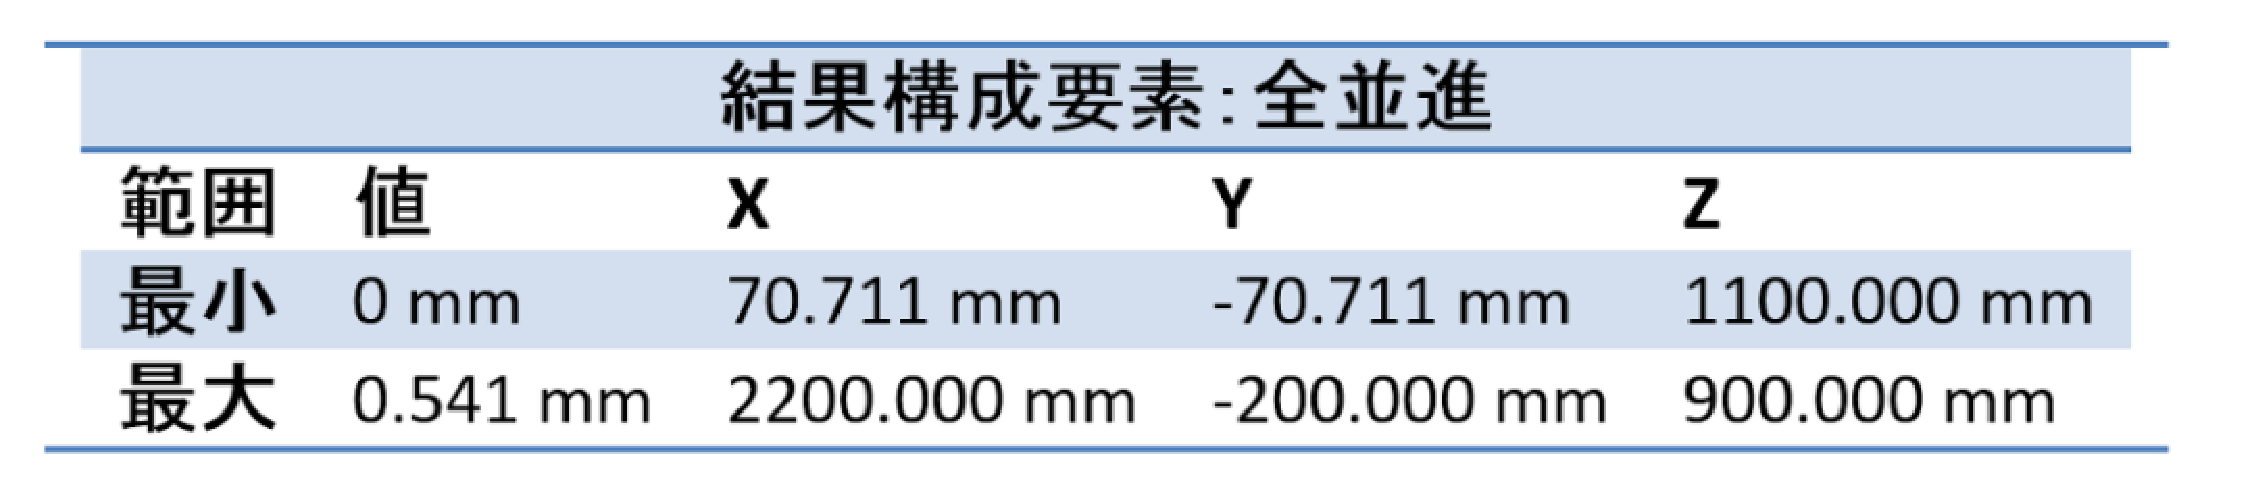
\includegraphics[height=2.5cm]{img/eps/default-heni-result.eps}
    \end{tabular}
    \caption{基準ロボットの変位解析結果}
    \label{default-heni-result}
  \end{center}
\end{figure}

シミュレーションによって数値的に得た変位の結果と,解析的に計算した変位の結果を比較する.

材料を引っ張った際の垂直応力\(\sigma\)と垂直ひずみ\(\epsilon\)の関係は縦弾性係数\(E\)を用いて,式\ref{suityoku}と表せる.

\begin{eqnarray}
  \epsilon &=& \frac{1}{E}\sigma
  \label{suityoku}
\end{eqnarray}

また,材料を引っ張った際のせん断応力\(\tau\)とせん断ひずみ\(\gamma\)の関係は,横弾性係数\(G\)を用いて,式\ref{sendan}と表せる.

\begin{eqnarray}
  \gamma &=& \frac{1}{G}\tau
  \label{sendan}
\end{eqnarray}

しかし,式\ref{suityoku}及び式\ref{sendan}を使用して計算した場合,SolidEdgeのシミュレーション結果によって出力された値とは一致しなかった.

その理由は,式\ref{suityoku}及び式\ref{sendan}で求められるのは応力をかけた場合のひずみであり,変位とは異なるものだからである.

そこで,カスティリアノの定理を用いて変位の理論解を計算することにした.

カスティリアノの定理とは,ひずみエネルギー\(U\)を,荷重\(W_{i}\)で偏微分することで,その荷重が作用している点での荷重の作用方向の変位\(v_{i}\)を得ることが出来るという定理であり,式\ref{castigliano}で表される.

\begin{eqnarray}
  \frac{\partial U}{\partial W_{j}} = v_{j}
  \label{castigliano}
\end{eqnarray}

ここで,弾性エネルギー\(U\)は,曲げモーメント\(M\)及び縦弾性係数\(E\),そして断面二次モーメントを\(I\),アームの回転中心からアーム先端までの距離を\(l\)とした時,式\ref{danseienergy}となる.

\begin{eqnarray}
  U =   \int_0^l \frac{M^2}{2EI} dx  
  \label{danseienergy}
\end{eqnarray}

この弾性エネルギー\(U\)の値をカスティリアノの定理に適用すると,式\ref{castigliano-calc}を得る.

\begin{eqnarray}
  v_{j} = \frac{\partial U}{\partial W_{j}} = \frac{\partial}{\partial W_{j}}\int_0^l \frac{M^2}{2EI} dx = \int_0^l \frac{M}{EI}\frac{\partial M}{\partial W_{j}}dx
  \label{castigliano-calc}
\end{eqnarray}

ゆえに,今回のたわみ\(v\)は,先ほど求めた曲げモーメント及びその偏微分値を使用して計算すると式\ref{tawami-calc}となる.ただし,\(R_1\)はアーム中心部に設置したブレードによる荷重,\(l_1\)はアームの回転中心とアーム中心部に設置したブレードとの距離,\(R_2\)はアーム先端部に設置したブレードによる荷重,\(l_2\)はアームの回転中心とアーム中心部に設置したブレードとの距離,\(W\)はアームの自重による荷重,\(l\)はアームの回転中心からアーム先端までの距離である.

\begin{eqnarray}
  v &=& \int_0^l \frac{M}{EI}\frac{\partial M}{\partial W_{j}}dx \nonumber \\
    &=& -\frac{1}{EI} \Bigl( -\frac{R_1}{3}l_1^3 - \frac{R_2}{3}l_2^3 - \frac{W}{8}l^4\Bigr)
  \label{tawami-calc}
\end{eqnarray}

また,断面二次モーメント\(I\)は直方体のY方向長さ\(b=0.4[\rm m]\)と,直方体のZ方向長さ\(h=0.2[\rm m]\)を使って,式\ref{danmen-niji}のように求められる.

\begin{eqnarray}
  I &=& \frac{bh^3}{12} \nonumber \\
    &=& \frac{0.4*0.2^3}{12} \nonumber \\
    &=& 0.0002667
  \label{danmen-niji}
\end{eqnarray}

式\ref{tawami-calc}に,各種値,\(R_1=117.6[\rm N]\),\(l_1=1.0[\rm m]\),\(R_2=117.6[\rm N]\),\(l_2=2.0[\rm m]\),\(W=485.8*9.81\),\(l=2.0[\rm m]\),\(I=0.0002667[\rm m^4]\),そしてアルミニウム1060の縦弾性係数\(E=68.60[\rm GPa]\)を代入すると,変位\(v[\rm mm]\)は,式\ref{calc-heni}となる.

\begin{eqnarray}
  v &=& -\frac{1}{EI} \Bigl( -\frac{R_1}{3}l_1^3 - \frac{R_2}{3}l_2^3 - \frac{W}{8}l^4\Bigr) \nonumber \\
    &=& -\frac{1}{18.26 * 10^6} \Bigl( -\frac{117.6}{3}1^3 - \frac{117.6}{3}2^3 - \frac{485.8*9.81}{8}2^4\Bigr) \nonumber \\
    &=& -\frac{1}{18.26 * 10^6} (-9875.1) \nonumber \\
    &=& 0.0005408[\rm m]
  \label{calc-heni}
\end{eqnarray}

となり,カスティリアノの定理を用いて計算した理論的な変位は0.0005408{[}m{]}=0.5408{[}mm{]}となった.Solid
Edgeのシミュレーション結果は0.541{[}mm{]}であったため,この解析結果は正しいことが分かる.

\subsection{基準ロボットの機構解析}\label{ux57faux6e96ux30edux30dcux30c3ux30c8ux306eux6a5fux69cbux89e3ux6790}

ここでは,基準ロボットの機構解析を行っていく.

ロボットアームに対して,基準座標系\(\Sigma_0\),リンク座標系\(\Sigma_1\),及び手先座標系\(\Sigma_E\)を記述したのが図\ref{basis-tesaki}である.

\begin{figure}[htbp]
  \begin{center}
    \begin{tabular}{c}
      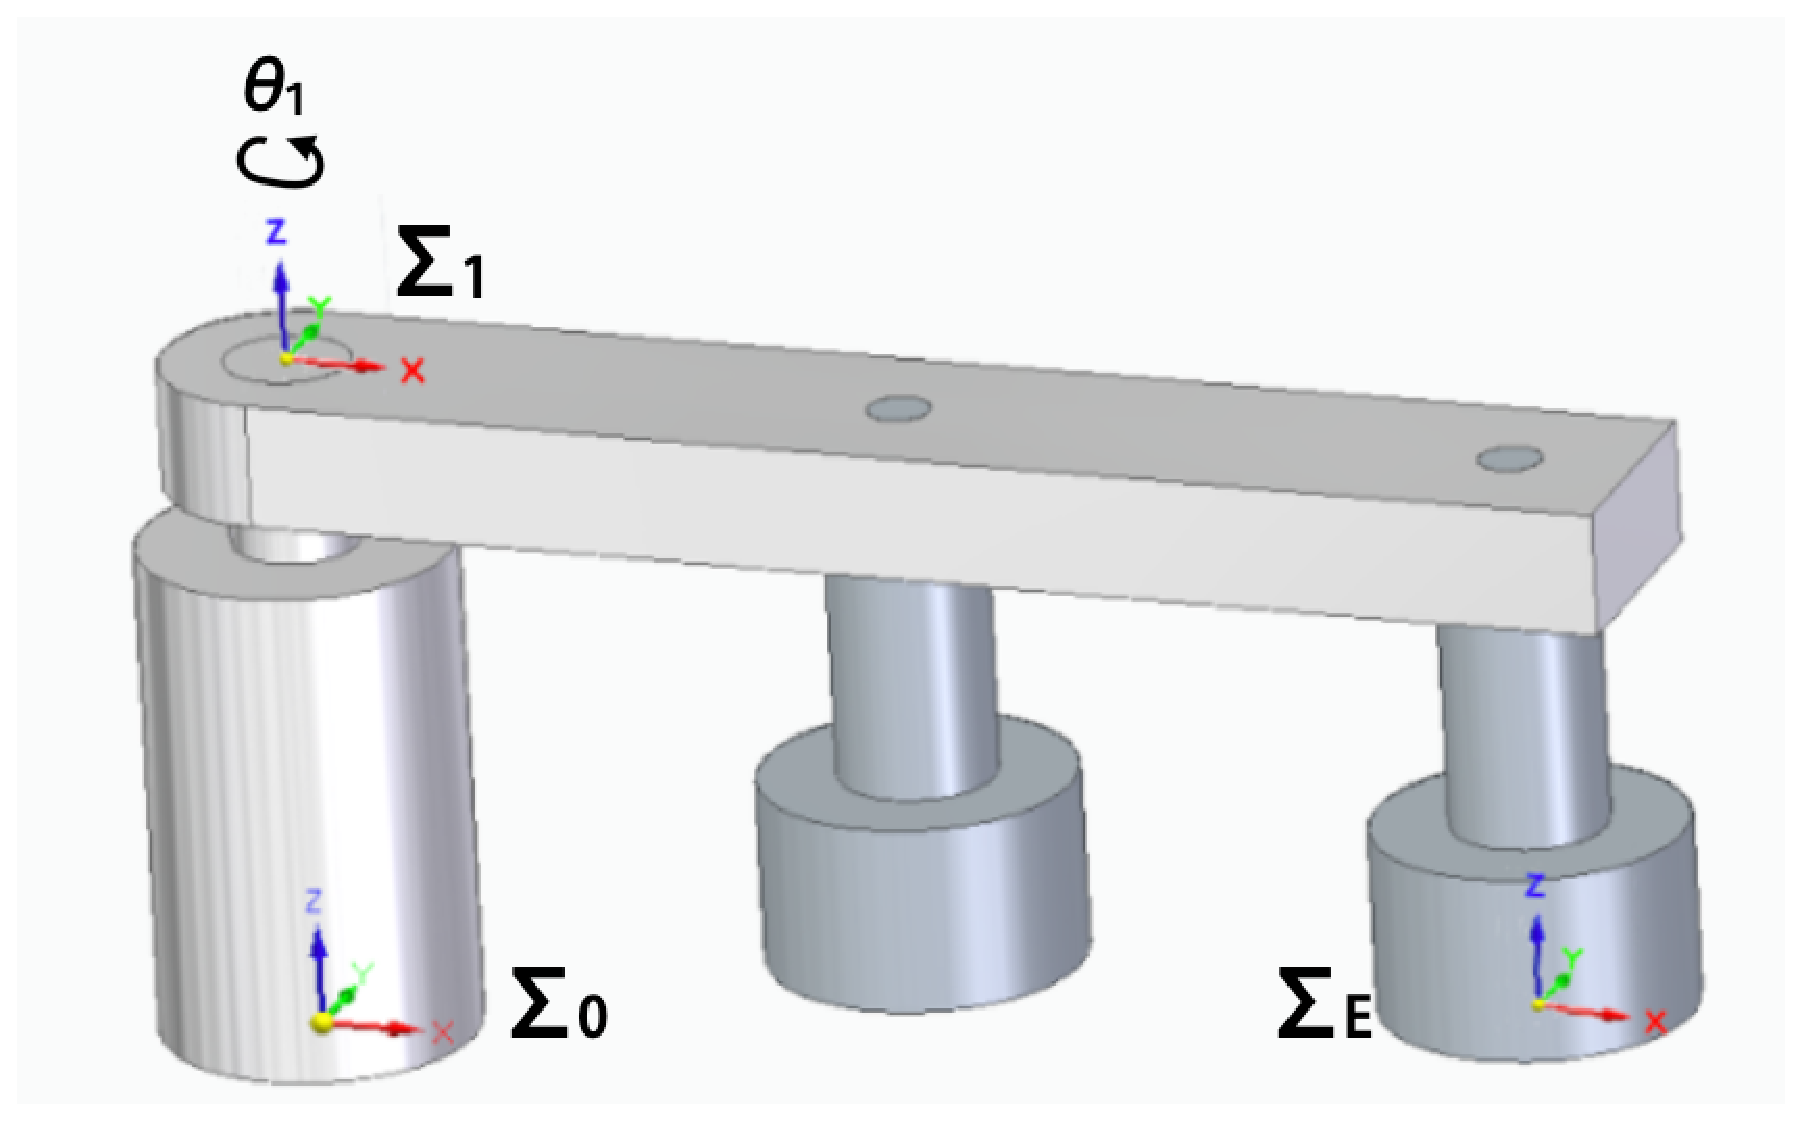
\includegraphics[height=5.0cm]{img/eps/basis-dh.eps}
    \end{tabular}
    \caption{基準ロボットの各種座標系}
    \label{basis-tesaki}
  \end{center}
\end{figure}

このロボットアームのリンクパラメータをDH記法を用いて書くと表\ref{basis-dh-link}となる.
今回,手先としてアーム先端のブレード部分を選んだ.

\begin{table}[htb]
\caption[]{リンクパラメータ}
  \begin{center}
    \begin{tabular}{|c|c|c|c|c|} \hline
      $i$ & $a_{i-1}$ & $\alpha_{i-1}$ & $d_i$ & $\theta_i$\\ \hline \hline
      1 & 0 & 0 & 1100[mm] & ($\theta_1$) \\ \hline
      2 & 2000[mm] & 0 & -900[mm] & 0 \\ \hline
    \end{tabular}
    \label{basis-dh-link}
  \end{center}
\end{table}

SimXpertを使用して,今回作成したアームロボットの関節回転角度を求めた結果を図\ref{basis-kaiten}に示す.

\begin{figure}[htbp]
  \begin{center}
    \begin{tabular}{c}
      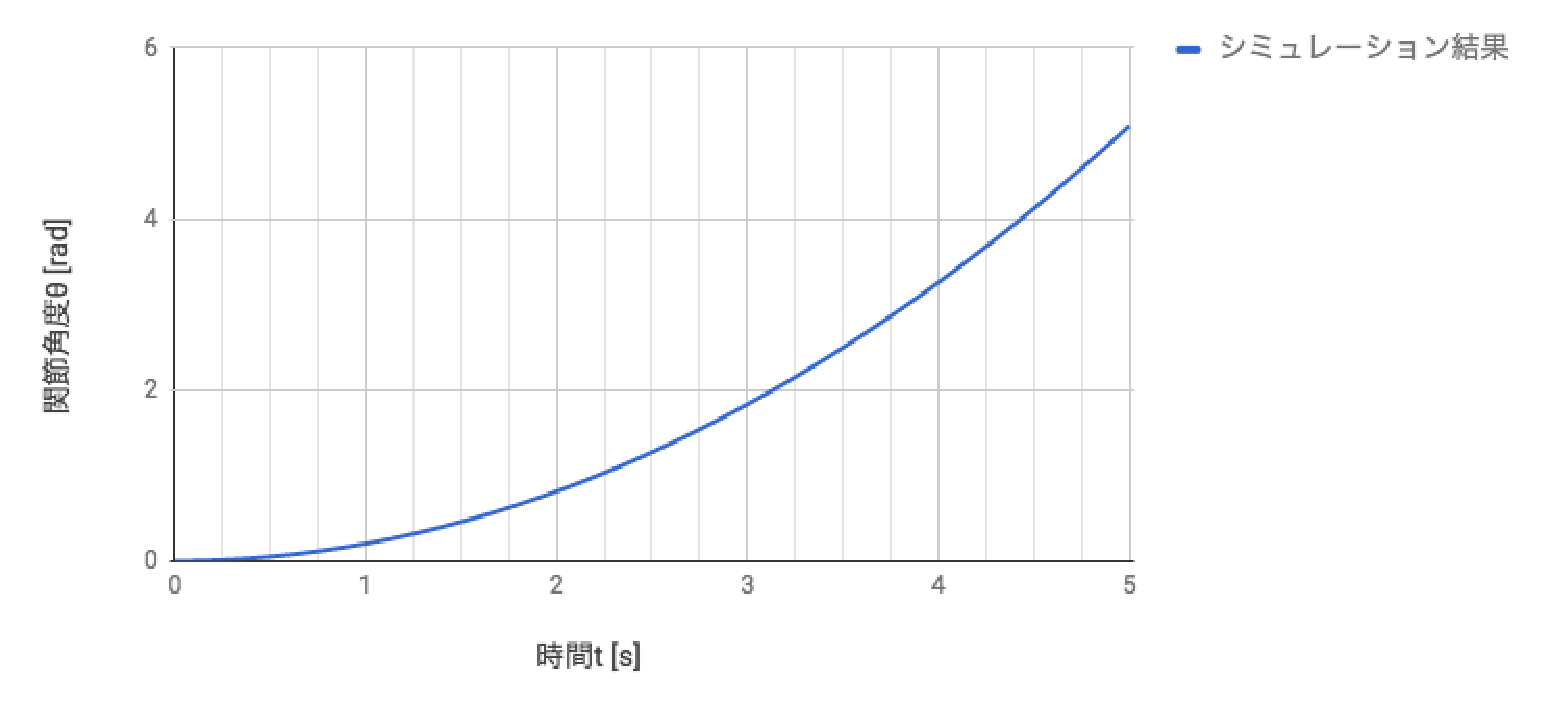
\includegraphics[height=4.5cm]{img/eps/basis-kaiten2.eps}
    \end{tabular}
    \caption{基準ロボットのアームの関節回転角}
    \label{basis-kaiten}
  \end{center}
\end{figure}

図\ref{basis-kaiten}のグラフは,横軸に経過時間,縦軸に回転角{[}rad{]}を取っている.

このシミュレーションで得られたアームロボットの回転角度を,理論解と比較する.

アームの慣性モーメントを\(I\),アームを回転させるトルクを\(\tau\),回転角を\(\theta\)とした時に,式\ref{kaiten-houteisiki}が成り立つ.

\begin{eqnarray}
  \tau &=& I \frac{d^2 \theta}{d t^2}
  \label{kaiten-houteisiki}
\end{eqnarray}

式\ref{kaiten-houteisiki}に,今回の関節駆動トルク\(\tau=393\),そして慣性モーメント\(I=751.9\)を代入すると,式\ref{kaiten-houteisiki-calc}となる.

\begin{eqnarray}
  393 &=& 751.9 \frac{d^2 \theta}{d t^2}
  \label{kaiten-houteisiki-calc}
\end{eqnarray}

式\ref{kaiten-houteisiki-calc}は,時間に関する2階微分であるので,角速度及び角度の初期値を0として両辺時間で2度積分することで微分方程式を解くと,式\ref{basis-deg}の角度の関数を得る.

\begin{eqnarray}
  \theta = 0.2613t^2
  \label{basis-deg}
\end{eqnarray}

先ほどSimXpertで得られたシミュレーションの結果と,式\ref{basis-deg}で求めた\(\theta\)に関する式を比較したのが図\ref{compare}である.

\begin{figure}[htbp]
  \begin{center}
    \begin{tabular}{c}
      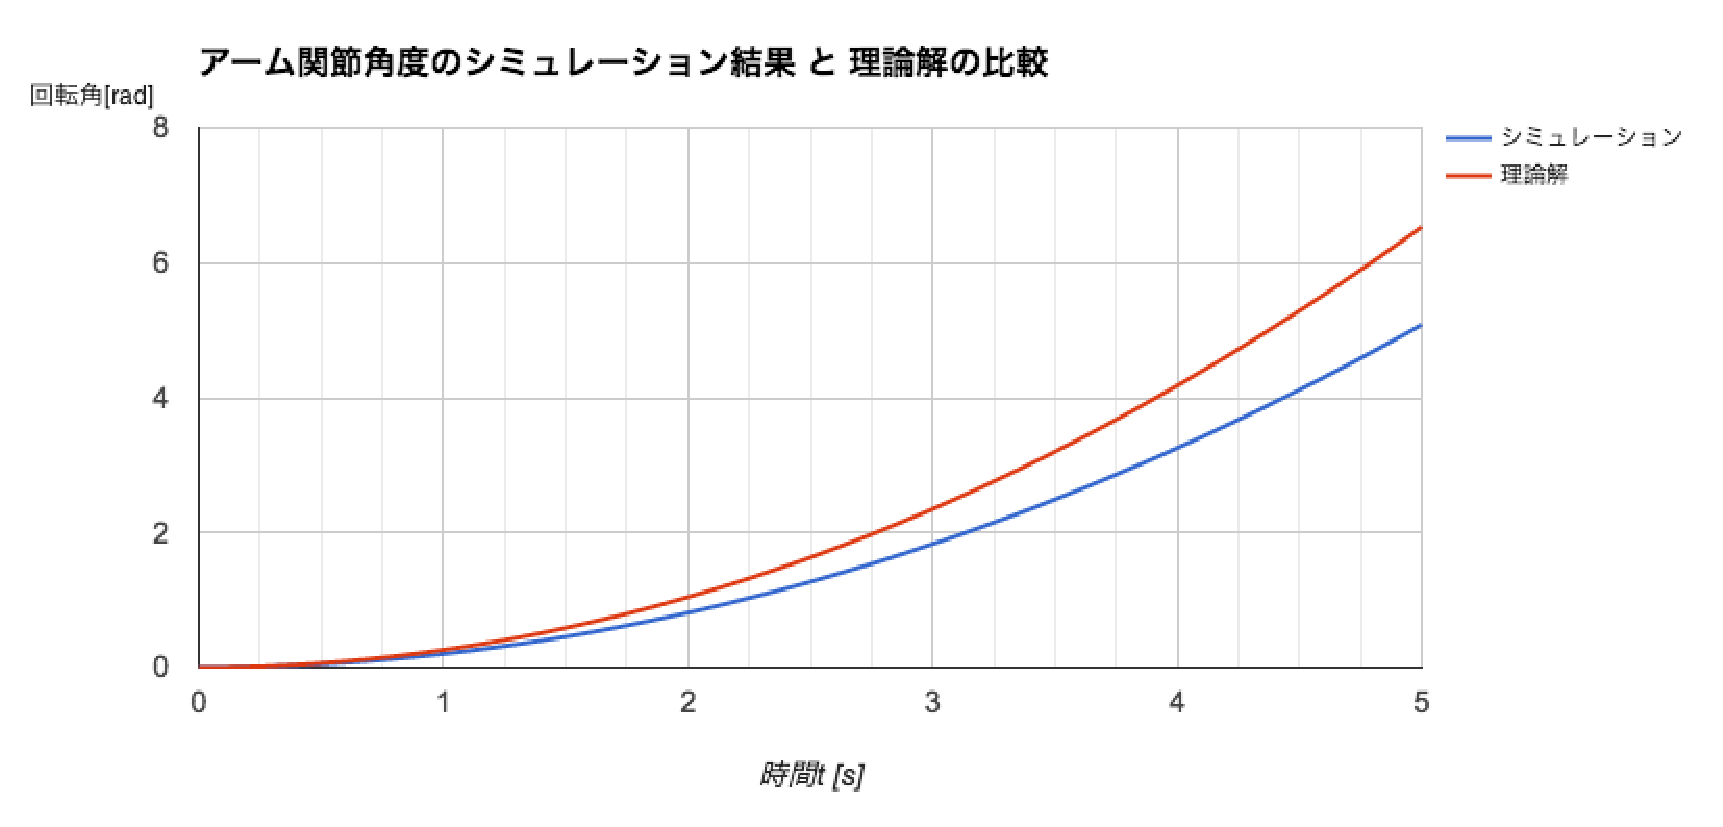
\includegraphics[height=7.5cm]{img/eps/compare.eps}
    \end{tabular}
    \caption{シミュレーション結果と理論解の回転角度の比較}
    \label{compare}
  \end{center}
\end{figure}

理論解のほうが少し回転角が大きくなっていることが図\ref{compare}より分かる.これは,シミュレーション時には,ブレード部分の質量を考慮しているが,理論解を出す場合は単純化のためにアーム部分のみを考えている.
その為,シミュレーションを行ったときのほうがブレード部分だけ慣性モーメント及び質量が大きくなっている.ゆえに,シミュレーション結果のほうが理論解に比べて回転量が小さくなってしまったと考えられる.
この関節角度のシミュレーション結果を最小二乗法を用いて2次の多項式近似を行うと,式\ref{basic-niji-kinji}を得ることが出来る.

\begin{eqnarray}
  \frac{d\theta}{dt} &=& 0.203t^2+0.00131x-0.000527 \nonumber \\
  &\approx& 0.203t^2
  \label{basic-niji-kinji}
\end{eqnarray}

式\ref{basic-niji-kinji}で得た関節加速度を使用し,手先加速度及び手先速度の理論値を計算し,シミュレーション結果と比較する.

手先加速度に関して,SimXpertを使って求めたものは手先加速度のノルムがどんどん上がっていた.同じ大きさのトルクを掛け続けた場合,手先加速度のノルムは常に一定となるはずであり,図\ref{basis-tesaki-kasokudo}の手先加速度のシミュレーション結果は,明らかに間違っているといえる.そこで,この手先加速度のシミュレーション結果より議論するのではなく,次に示す手先速度のシミュレーション結果を元にして手先加速度を割り出すという方法を取ることにする.

SimXpertより出力された手先速度を図\ref{basis-tesaki-sokudo}に示す.

\begin{figure}[htbp]
  \begin{center}
    \begin{tabular}{c}
      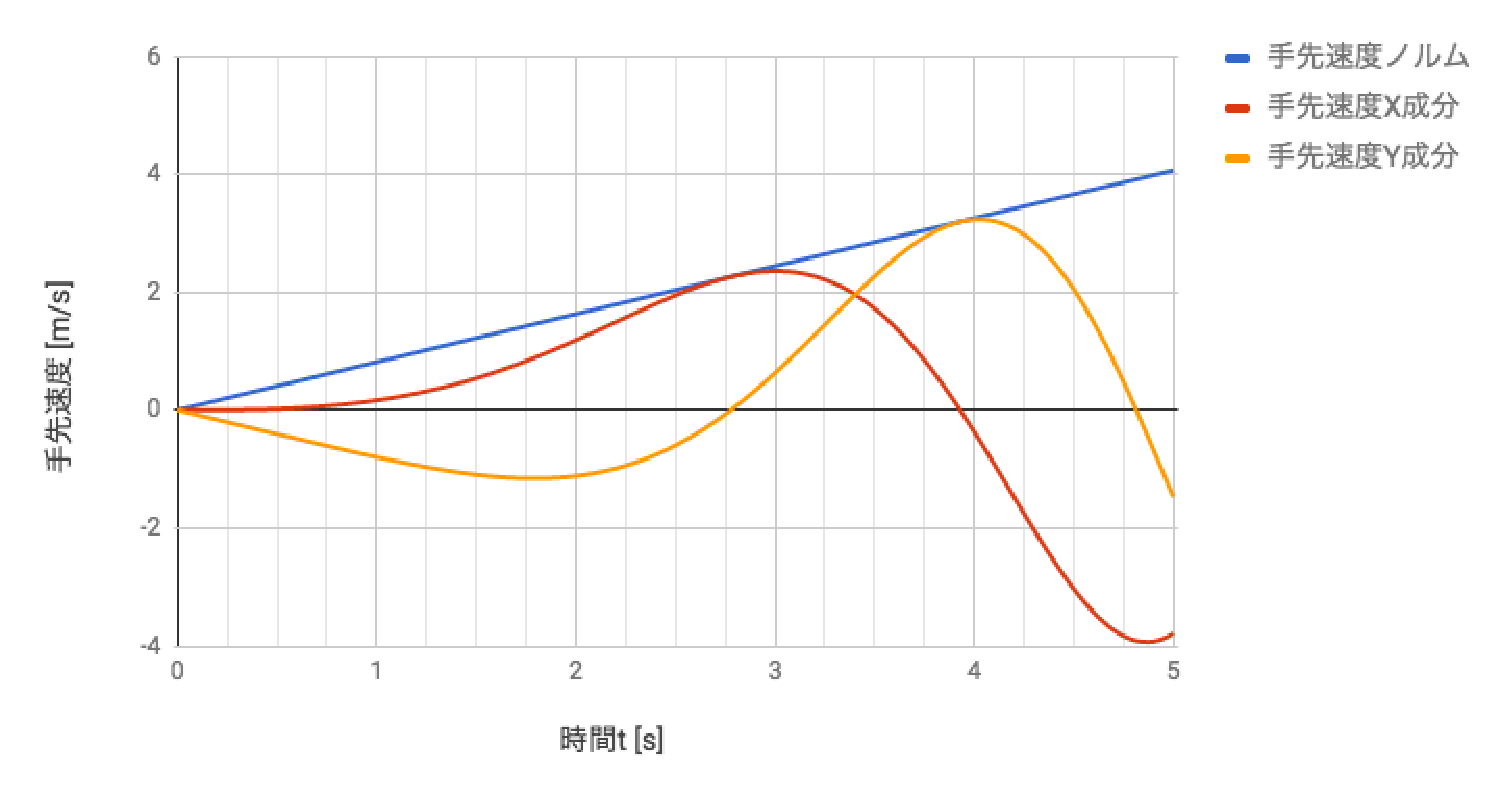
\includegraphics[height=5.5cm]{img/eps/basis-tesaki-sakudo2.eps}
    \end{tabular}
    \caption{手先速度のシミュレーション結果}
    \label{basis-tesaki-sokudo}
  \end{center}
\end{figure}

次に,この手先速度のシミュレーション結果の妥当性を理論解と比較することで検証する.
先ほど,式\ref{basic-niji-kinji}で,\(\theta = 0.203t^2\)を得た.

ゆえに,角速度\(\frac{d\theta}{dt}\)は式\ref{basic-niji-kinji}を両辺\(t\)で時間微分することで得られ,式\ref{basic-ddeg}となる.

\begin{eqnarray}
  \frac{d\theta}{dt} = 0.406t
  \label{basic-ddeg}
\end{eqnarray}

ここで,角速度\(\frac{d\theta}{dt}\)と手先速度の大きさ\(v\)の間には,式\ref{hand-vel}の関係がある.ただし,回転中心と手先間の距離を\(r\)と置いた.

\begin{eqnarray}
  v &=& r\frac{d\theta}{dt}
  \label{hand-vel}
\end{eqnarray}

式\ref{basic-ddeg},及び式\ref{hand-vel}より,手先速度の大きさの理論解は式\ref{b-hand-velocity}となる.

\begin{eqnarray}
  v &=& r(0.406t) \nonumber \\
    &=& 2(0.406t) \nonumber \\
    &=& 0.812t
  \label{b-hand-velocity}
\end{eqnarray}

ゆえに,手先速度の理論解は\(v=0.812t\)と求まった.

SimXpertによって得られた手先速度のシミュレーション結果を最小二乗法によって1次関数近似を行うと,式\ref{teaki-kinji}を得る.

\begin{eqnarray}
 v &=& 0.813t+0.00147 \nonumber \\
 &\approx& 0.813t 
  \label{teaki-kinji}
\end{eqnarray}

手先速度のシミュレーション結果によって得られた式\ref{teaki-kinji}と式\ref{b-hand-velocity}の理論解は一致しており,シミュレーション結果が正しいと考えられる.

ここで,この手先速度を時間微分したものが手先加速度であるため,手先加速度として\(0.813[\rm m/s^2]\)を得る.

手先加速度の理論解および数値解のグラフを図\ref{basic-acc}に示す.

\begin{figure}[htbp]
  \begin{center}
    \begin{tabular}{c}
      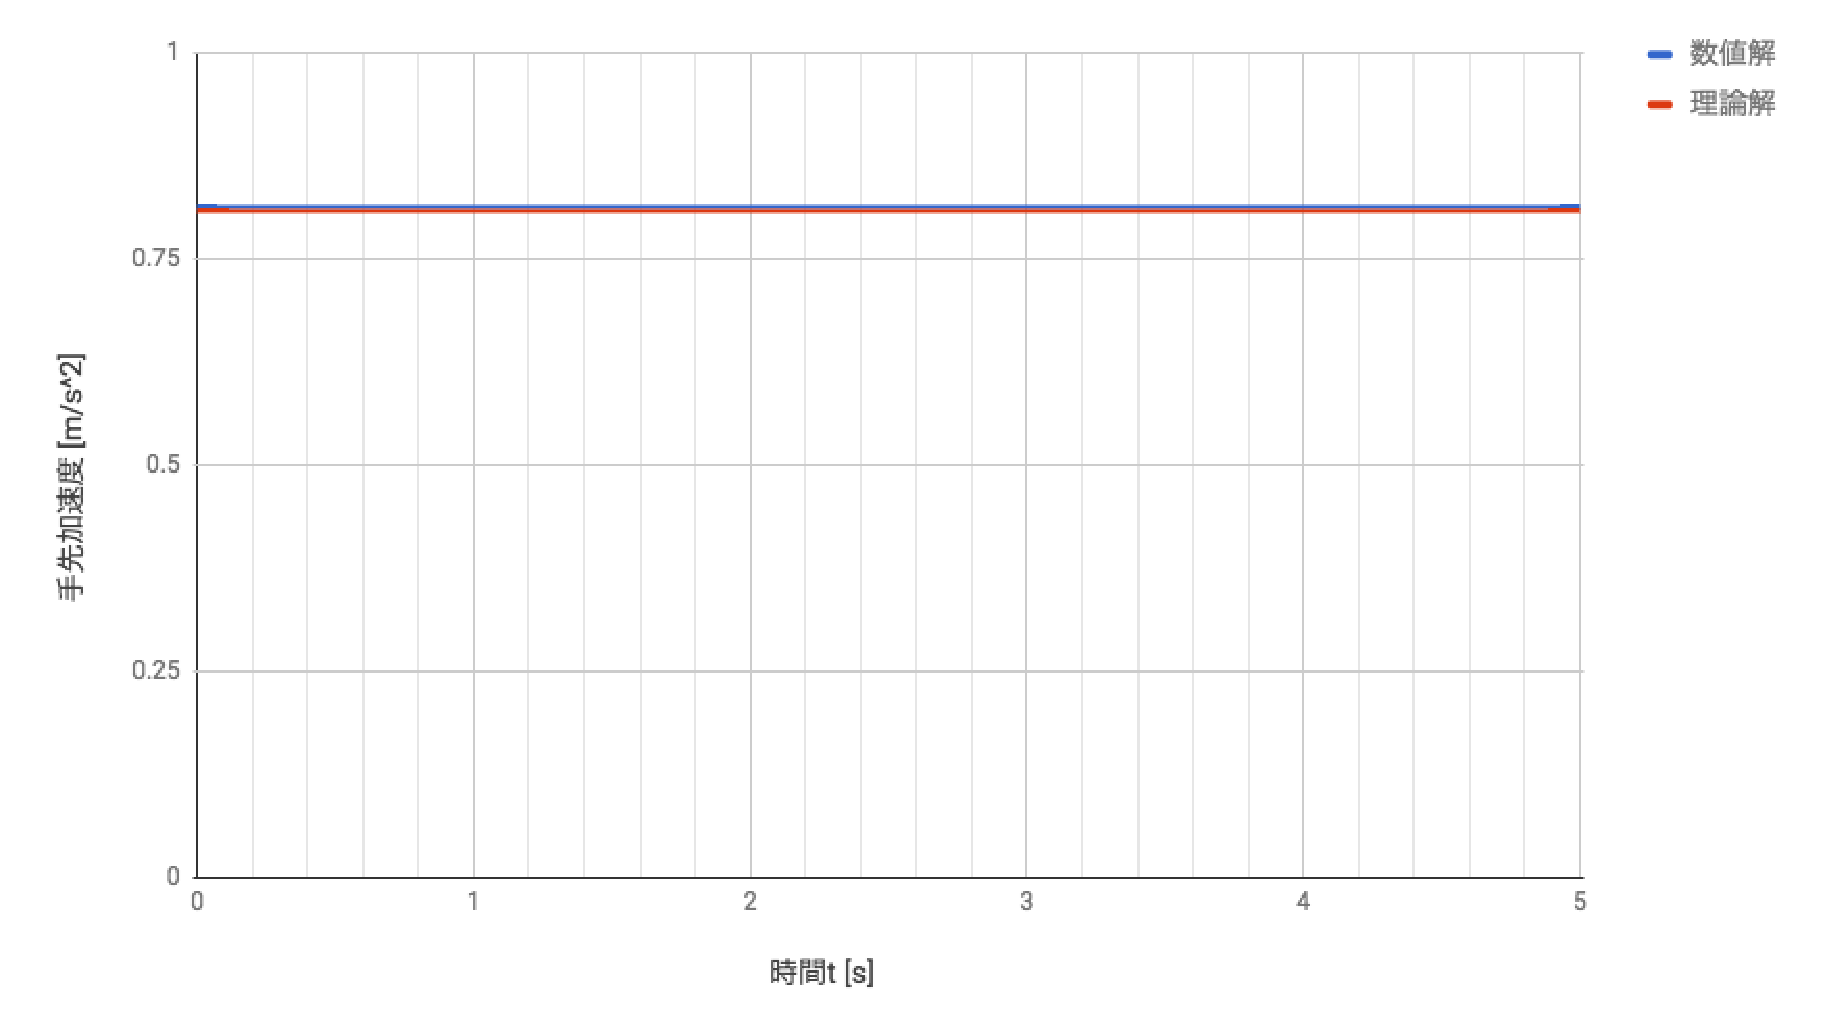
\includegraphics[height=5.5cm]{img/eps/basis-acc.eps}
    \end{tabular}
    \caption{手先加速度の理論解と数値解の比較}
    \label{bacic-acc}
  \end{center}
\end{figure}
